% chapter 4 section 2

\section{电流}

\subsection{欧姆定律}
\label{subsec:欧姆定律}

本节内容较为基础,在此只逐条列举重要知识点。

\subsubsection{电流}

\begin{itemize}
    \item 描述:由电荷的定向移动形成
    \item 方向:正电荷的流动方向,或者负电荷流动的反方向
    \item 大小:单位时间内流过导体截面的电量
    \item 定义式1(宏观):
    \begin{equation*}
        I=\frac{\Delta Q}{\Delta t}
    \end{equation*}
    \item 定义式2(微观)\footnote{n为单位体积的电子密度,v为电子移动速度,S为导体截面积}:
    \begin{equation*}
        I=neSv
    \end{equation*}
    \item 单位:安培(A)
\end{itemize}

\subsubsection{欧姆定律}

\begin{equation*}
    V=IR
\end{equation*}
\begin{itemize}
    \item 描述:流过导体的电流与加在其两端电压的大小成正比
    \item 电阻R:日文为電気抵抗
    \begin{figure}[ht!]
        \centering
        \begin{circuitikz}[european]
            \draw (0,0) to[R=$3k\Omega$,o-o] (2,0);
        \end{circuitikz}
    \end{figure}
    \begin{itemize}
        \item 单位:欧姆($\Omega$)
        \item 定义式:$R=\rho\frac{l}{S}$
        \item 串联:$R=R_1+R_2$
        \item 并联:$\frac{1}{R}=\frac{1}{R_1}+\frac{1}{R_2}$
    \end{itemize}
\end{itemize}

\subsubsection{焦耳热}

\begin{itemize}
    \item 本质:电场力对电子的做功
    \item 公式:
    \begin{equation*}
        Q=VIt=I^2Rt=\frac{V^2}{R}t
    \end{equation*}
    \item (电)功率:
    \begin{equation*}
        W=VI=I^2R=\frac{V^2}{R}
    \end{equation*}
\end{itemize}

\subsection{直流电路}
\label{subsec:直流电路}

\paragraph{基尔霍夫定律}适用于任何闭合电路,是解决复杂电路问题的重要手段。
\begin{itemize}
    \item 电流表述:回路中任意一个节点都满足$I_\textrm{流入}=I_\textrm{流出}$
    \item 电压表述:任意一个闭合回路都满足$V_\textrm{下降}=V_\textrm{上升}$
\end{itemize}
\begin{figure}[ht!]
    \centering
    \begin{circuitikz}[european]
        \draw (0,0)
        to[battery1=$V_1$, invert] (2,0)
        to[R=$R_1$] (4,0)
        to[short, i=$I_1$] (6,0)
        to[short] (6,4)
        to[short, i=$I_3$] (3,4)
        to[R=$R_3$] (0,4)
        to[short] (0,0);
        \draw (0,2)
        to[battery1=$V_2$, invert] (2,2)
        to[R=$R_2$] (4,2)
        to[short, i=$I_2$] (6,2);

        \draw[color=gray, opacity=0.5, thick, -latex] (0.1,-0.1) -- (6.2,-0.1) -- (6.2,4.1) -- (-0.2,4.1) -- (-0.2,-0.1);
        \draw[color=gray, opacity=0.5, thick, -latex] (0.4,2.1) -- (5.8,2.1) -- (5.8,3.9) -- (0.2,3.9) -- (0.2,2.1);
    \end{circuitikz}
    \caption{基尔霍夫定律}
\end{figure}
对于图示的两条闭合回路,则可以列如下等式。
\begin{itemize}
    \item $+V_1-R_1I_1-R_3I_3=0$
    \item $+V_2-R_2I_2-R_3I_3=0$
    \item $I_1+I_2=I_3$
\end{itemize}

\paragraph{电池内阻}在一般问题中题目常常将电池视作理想的供能元件,但事实上电池内部也存在电阻,简称为电池内阻。同时,当我们使用电压表测电压时,即便接在电池两端测量,得到的结果也是外路的数值,即无法直接测定电池的实际起电力。
\begin{figure}[ht!]
    \centering
    \begin{circuitikz}[european]
        \draw (0,0)
        to[battery1=$E$, invert]  (2,0)
        to[R=$r$] (4,0)
        to[short] (4,4)
        to[R=$R$] (0,4)
        to[short] (0,0);
        \draw (0,2)
        to[voltmeter, *-*] (4,2);
        \fill[fill=gray, opacity=0.3] (-0.2,-0.5) rectangle (4.2,1.2);
    \end{circuitikz}
    \caption{电池内阻}
\end{figure}
对上述简化电路列基尔霍夫方程可得
\begin{gather*}
    E=rI+V\\
    V(I)=-rI+E
\end{gather*}
因此,只要确定了该电路的$V-I$直线后即可通过纵截距间接求得电池实际的起电力。

\paragraph{惠斯通电桥}日文为ホイートストンブリッジ,是一个测量未知电阻阻值的结构。其中已知$R_1$与$R_2$,$R_3$是一个阻值可调的可变电阻,当图中电流表示数为0时,则$R_4$值可求。
\begin{figure}[ht!]
    \centering
    \begin{circuitikz}[european]
        \draw (0,0)
        to[short] (0,3)
        to[R=$R_1$] (3,3)
        to[vR=$R_3$] (6,3)
        to[short] (6,0)
        to[battery1, invert]  (0,0);
        \draw (0,1.5)
        to[R=$R_2$] (3,1.5)
        to[R=$R_4$] (6,1.5);
        \draw (3,1.5) to[ammeter, *-*] (3,3);
    \end{circuitikz}
    \caption{惠斯通电桥}
\end{figure}

当电流表示数为0,即其两端没有电势差时,$R_1$和$R_2$消耗的电压相同、$R_3$和$R_4$消耗的电压相同,因此可列方程
\begin{equation*}
    \frac{R_1}{R_2}=\frac{R_3}{R_4}
\end{equation*}

\paragraph{非线性电阻}一般用电器的电阻并非恒定,而是会随着诸如温度等物理条件变化,我们称其为非线性电阻。
\begin{figure}[ht!]
    \centering
    \begin{minipage}{0.48\textwidth}
        \centering
        \begin{circuitikz}[european]
            \draw (0,0)
            to[short, i=$I$] (0,1.5)
            to[lamp=$V$] (2,1.5)
            to[R=$1\Omega$] (4,1.5)
            to[short] (4,0)
            to[battery1=$4V$, invert] (0,0);
        \end{circuitikz}
    \end{minipage}
    \begin{minipage}{0.48\textwidth}
        \centering
        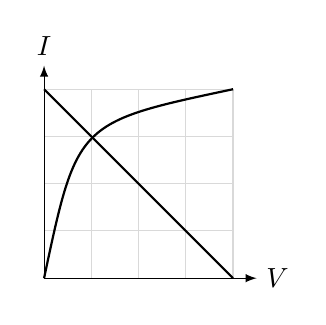
\begin{tikzpicture}[scale=0.6]
            \draw[color=gray!30, step=1] (0,0) grid (4,4);
            \draw[-latex] (0,0) -- (4.5,0) node[right] {$V$};
            \draw[-latex] (0,0) -- (0,4.5) node[above] {$I$};
            \draw[thick] (0,0) .. controls (0.7,3.3) .. (4,4);
            \draw[thick] (0,4) -- (4,0);
        \end{tikzpicture}
    \end{minipage}
    \caption{非线性电阻}
\end{figure}
关于整个回路列基尔霍夫方程可得:$V+I=4$,也就是说回路中的灯泡同时满足这个等式和它自己的变化规律。数形结合,两条线的交点即为唯一符合条件的电压值与电流值。
